% Copyright (C) 2007 Technical University of Liberec.  All rights reserved.
%
% Please make a following reference to Flow123d on your project site if you use the program for any purpose,
% especially for academic research:
% Flow123d, Research Centre: Advanced Remedial Technologies, Technical University of Liberec, Czech Republic
%
% This program is free software; you can redistribute it and/or modify it under the terms
% of the GNU General Public License version 3 as published by the Free Software Foundation.
%
% This program is distributed in the hope that it will be useful, but WITHOUT ANY WARRANTY;
% without even the implied warranty of MERCHANTABILITY or FITNESS FOR A PARTICULAR PURPOSE.
% See the GNU General Public License for more details.
%
% You should have received a copy of the GNU General Public License along with this program; if not,
% write to the Free Software Foundation, Inc., 59 Temple Place - Suite 330, Boston, MA 021110-1307, USA.
%
%%%%%%%%%%%%%%%%%%%%%%%%%%%%%%%%%%%%%%%%%%%%%%%%%%%%%%%%%%%%%%%%%%
%
% use PDFLatex to compile this
%

\documentclass[a4paper]{article}

% our own flow_doc.sty
%\usepackage{flow_doc}

%\usepackage{rotating}
%\usepackage{pdflscape}

\usepackage{amssymb, amsmath, amsthm}
\newtheorem{theorem}{Theorem}


\usepackage{array}
\usepackage{longtable}
\usepackage[usenames,dvipsnames]{color}   %colors
%\usepackage{colortbl}   %colorful tables
\usepackage{tabularx}
\usepackage{graphicx} %[dvips]
% it is note used \usepackage{cooltooltips}

%these two can be found in caption package
%\usepackage{caption}
%\usepackage{subcaption}

\usepackage[numbers]{natbib}

%\usepackage{fancyvrb}   % extended verbatim environments (for examples of IO files)

%\usepackage{multicol}
\usepackage{etoolbox}


%%%%%%%%%%%%%%%%%%%%%%%%%%%%%%%%%%%%%%%%%%%%%%%%%%%%%%%%%%%%%%%%%%%%%%%%%%%%
% macro for units 
\def\UNIT#1#2{\ifstrempty{#2}{}{%
\ifstrequal{#2}{1}{\mathrm{#1}}{\mathrm{#1}^{#2}}%
}}
\def\units#1#2#3{\ifstrempty{#1#2#3}{$[-]$}{$[ \UNIT{kg}{#1}\UNIT{m}{#2}\UNIT{s}{#3} ]$}}       %with brackets
\def\unitss#1#2#3{\ifstrempty{#1#2#3}{$-$}{$ \UNIT{kg}{#1}\UNIT{m}{#2}\UNIT{s}{#3} $}}  %without brackets


\newcommand{\vari}[1]{{\it #1}}
\newcommand{\ditem}[2]{\item[\vari{#1} {\tt #2}]}
\newenvironment{fileformat}{\tt\begin{flushleft}}{\end{flushleft}}

%%%%%%%%%%%%%%%%%%%% specific math macros
\def\prtl{\partial}
\def\vc#1{\mathbf{\boldsymbol{#1}}}     % vector
\def\tn#1{{\mathbb{#1}}}    % tensor
\def\abs#1{\lvert#1\rvert}
\def\Abs#1{\bigl\lvert#1\bigr\rvert}
\def\div{{\rm div}}
\def\ep{\varepsilon}
\def\Lapl{\Delta}
\def\grad{\nabla}
\def\Real{{\mathbf R}}
\def\d {\,{\rm d}}
\def\Natural{\mathbf N}
\def\norm#1{\|#1\|}
\def\yy{{\vc y}}
\def\ul{\underline}
\def\ol{\overline}

\newcommand{\note}[2]{{\color{blue} \textbf{ #1:} \textit{#2}}}
%% ini_table members
%%%%%%%%%%%%%%%%%%%% specific math macros


%%%%%%%%%%%%%%%%%%%%%%%%%%%%%%%%%%%%%%%%%%%%%%%%%%%%%%%%%%%%%%%%%%%%%%%%%%%%%%%%%%%%%%%%%%%%% BEGIN DOCUMENT
%% set specific page layout
%\addtolength{\textwidth}{2cm}
%\addtolength{\hoffset}{-1.5cm}
%\addtolength{\textheight}{4cm}
%\addtolength{\voffset}{-2.5cm}
\begin{document}

\section{Introduction}
\note{JB}{
\begin{itemize}
 \item Motivation, background (granite, impact of small scale to large scale)
 \item 2d domain, notation (figure with boundary perpendicular to fracture)
 \item Darcy flow, Solute transport equations, basic notation
\end{itemize}
}

Deep subsurface deposits in plutonic rock represents one of possible solution for final storage of nuclear waste. The primary reason is 
small hydraulic permeability of the bulk rock and thus slow migration of a possible leakage due to ground water flow.  On the other hand, 
granitoid formations contain fractures that may form a network of preferential paths with low volumetric water flow rate but with 
high velocity. The preferential paths pose a risk of fast transport of small amount of contaminant but in potentially dangerous concentrations.
The large scale effect of the small scale fractures is challenging for numerical simulations since direct discretization requires highly refined
computational mesh. One possible solution is to model fractures as lower dimensional objects and introduce their coupling with surrounding continuum.
\note{JB}{ Overview of other papers, namely: Martin et al \cite{martin_modeling_2005} (Darcy, classical derivation, numeric), Angot et al \cite{angot_asymptotic_2009} 
(Darcy, curved fracture, definition of trace operator for immersed fracture, finite volume scheme, convergence, our case not covered); Fumagalli and Scotti (transport, classical derivation).}


\note{JS}{
MODELLING FRACTURES AS INTERFACES - survey of works and results, lack of rigorous justification (either formal derivation or error estimates just for particular approximation scheme).
}

\note{JS}{
Only basic notation in introduction (2d domain, Darcy, AD eq.) remaining in derivation of abstract fracture model.
}

\begin{figure}[h]
\centering
\includegraphics[width=12cm]{figures/full_model_domain}
\label{fig:omegas}
\caption{The domain of the full model (left) and the reduced geometry (right).}
\end{figure}
\note{JB}{Technicality: Reduced geometry with $\Omega_m$ at original place better suites to derivation of the asymptotic model, but than we can not integrate $c_m-c_f$ over $\gamma$. ??}

We consider a bounded domain $\Omega \subset \Real^d$, $d=2,3$ with a Lipschitz boundary, see Figure \ref{fig:omegas} left). The domain $\Omega$ contains 
a fracture $\Omega_f:=\Omega\cap \big((-\delta/2,\delta/2)\times\Real^{d-1}\big)$ 
with the aperture $\delta>0$ surrounded by the matrix domain $\Omega_m:=\Omega\setminus\overline\Omega_f$. 
\note{JB}{$\Omega_m$ is not simply connected, thus not domain; are there some important consequences?}
The fracture interacts with the matrix domain on the interfaces 
$\gamma_1:=\Omega\cap\big( \{-\delta/2\}\times \Real^{d-1}\big)$ and 
$\gamma_2:=\Omega\cap\big( \{ \delta/2\}\times \Real^{d-1}\big)$. Normal vectors of these interfaces are denoted $\vc n_i$, $i=1,2$ with orientation out of the domain $\Omega_m$.
Further, we introduce reduced geometry (see Figure \ref{fig:omegas})
where the fracture domain is represented by the interface $\gamma:=\Omega\cap\big(\{0\}\times\Real^{d-1}\big)$ in its center. 

We are interested in a steady Darcy flow on domain $\Omega$:
\begin{subequations}
\label{eq:darcy_flow}
\begin{align}
    \div \vc q_p = f_p \mbox{ in }\Omega, \\
    \vc q_p = -\tn K \grad p, \\
    p=p_0\mbox{ on }\partial\Omega
\end{align}
\end{subequations}
where $\vc q_p$ is the Darcy flux, $f_p$ is the source density, $\tn K$ is the hydraulic conductivity tensor, $p$ is the piezometric head and $p_0$ is 
the piezometric head on the boundary.
Further, we consider also related solute transport equation:
\begin{subequations}
\label{eq:solute_transport}
\begin{align}
    \prtl_t (\theta c) + \div(q_c) = f_c \mbox{ in }\Omega,\\
    \vc q_c = c \vc q_p - \theta \tn D \grad c, \\
    \vc q_c \cdot \vc n= c_0 [\vc q_p \cdot \vc n]^-\mbox{ on }\partial\Omega
\end{align}
\end{subequations}
where $\theta$ is the porosity, $c$ is the solute concentration, $q_c$ is the total solute flux, 
$\tn D$ is the diffusion-dispersion tensor that in general depends on $q_h$, and 
$c_0$ is the solute concentration on the inflow part of the boundary.

Both transport processes are particular cases of an abstract advection-diffusion problem which admits an equivalent formulation
emphasizing the structure of the domain $\Omega$:
\begin{align}
  \label{eq:full:continuity}
  \prtl_t w_i + \div \vc j_i &= f_i&&  \text{in } \Omega_i,\ i=m,f,\\
  \label{eq:full:flux}
  \vc j_i &= - \tn A_i\grad u_i + \vc b_i w_i&& \text{in } \Omega_i,\ i=m,f,\\
  \label{eq:full:gammaDirichlet}
  u_i &= u_f&& \text{on } \gamma_i,\ i=1,2,\\
  \label{eq:full:gammaNeumann}
  \vc j_i \cdot \vc n &= \vc j_f \cdot \vc n&& \text{on } \gamma_i,\ i=1,2,
\end{align}
where $w_i=w_i(u_i)$ is the conservative quantity and $u_i$ is the principal unknown, $\vc j_i$ is the flux of $w_i$, $f_i$ is the source term,
$\tn A_i$ is the diffusivity tensor and $\vc b_i$ is the velocity field. 
Interior equations $(\ref{eq:full:continuity}-\ref{eq:full:gammaNeumann})$ are completed by general boundary conditions
\begin{align}
  \label{eq:full:outerDirichlet}
  u=u_D, \text{ on } \Gamma_D,\\
  \label{eq:full:outerNeumann}
  \vc j \cdot \vc n= w_N [\vc b \cdot \vc n]^- \mbox{ on }\Gamma_N\\
\end{align}
where $\Gamma_D$ and $\Gamma_N$ are the Dirichlet part and the Neumann part of the outer boundary $\prtl\Omega$.


In this paper we shall study the relation of the above problem to the so-called continuum-fracture problem on the reduced geometry.
Our goal is to justify the latter problem as an approximation of the first one in the case when the cross section $\delta$ is small.
In particular, we shall prove that
\[ \bar u - u_f \approx \delta\quad\mbox{and}\quad u_{|\Omega_m}-u_m \approx \delta^{3/2} \]
in a suitable sense.


The organization of the paper is as follows.
In the next section we present the formal derivation of the asymptotic model.
The main theoretical result on the error analysis is stated and proved in section \ref{sc:error_estimate}.
Finally, in section \ref{sc:numerics} we show numerical results which confirm the error estimates.



\section{Continuum-fracture model for the abstract problem}
\label{sc:ad_on_fractures}

In this section, we shall derive a model for the continuum-fracuter model of an abstract advection-diffusion process 
$(\ref{eq:full:continuity}-\ref{eq:full:outerNeumann})$
on the reduced geometry. This is done by integrating the equations $(\ref{eq:full:continuity}-\ref{eq:full:flux})$ on the fracture $\Omega_f$
in the normal direction and obtain their approximations on the surface $\gamma$ running through the middle of the fracture.

For the sake of simplicity, we will not write subscript $f$ for quantities on the fracture. 
By $x$, $\vc y$, we denote the normal and the tangential coordinate of a point in $\Omega_f$.
Accordingly, $\partial_x$, $\nabla_{\vc y}:=(0,\partial_{y_1},\ldots,\partial_{y_{d-1}})^\top$ stands for 
the crosswind and the tangential derivative, respectively. 
The symbol $\bar w:=\frac1\delta\int_{-\delta/2}^{\delta/2} w(x,\cdot)~dx$ will denote the integral mean of a function $w$ across the fracture opening.


We assume that the diffusive tensor $\tn A_f$ is symmetric positive definite 
with one eigenvector in the direction $\vc n$. Consequently the tensor has the form:
\[
 \tn A_f = \begin{pmatrix} 
            a_n & 0  \\
            0 & \tn A_t
       \end{pmatrix}
\]
Furthermore, we assume that $\tn A_f(x, \vc y)=\tn A_f(\vc y)$ is constant in the normal direction.
In order to make the procedure mathematically correct, we have to assume that the functions
$\prtl_x w$, $\prtl_x \grad_{\vc y} u$, $\prtl_x \vc b_{\vc y}$ are continuous and bounded on $\Omega_f$, moreover
Here and later on, 
$\vc b_x=(\vc b \cdot \vc n)\, \vc n$ is the normal part of the velocity field and $\vc b_{\vc y} = \vc b - \vc b_x$ is the tangential part.
The same notation will be used for normal and tangential part of the field $\vc j$.
\note{JB}{Assumption about dependence on time?}

We integrate \eqref{eq:full:continuity} over the fracture opening $[-\delta/2,\delta/2]$ and use approximations to get
\begin{equation}
    \label{eq:fracture_continuity}
   \prtl_t (\delta W) - \vc j_2 \cdot \vc n_2 - \vc j_1 \cdot \vc n_1 + \div \vc J = \delta F,
\end{equation}
where for the first term, we have used mean value theorem, first order Taylor expansion, 
and boundedness of $\prtl_x w$ to obtain approximation:
\[
    \int_{-\frac\delta2}^{\frac\delta2} w(x,\vc y) \d x=\delta w(\xi_{\vc y}, \vc y) = \delta W(\vc y) + O(\delta^2\abs{\prtl_x w}),
\]
where
\[
    W(\vc y):=w(0,\vc y)=w(u(0,\vc y))=:w(U(\vc y)).
\]
Next two terms in \eqref{eq:fracture_continuity} come from the exact integration 
of the divergence of the normal flux $\vc j_x$.
Integration of the divergence of the tangential flux $\vc j_{\vc y}$ gives the fourth term, where we introduced
\[
\vc J(\vc y) := \int_{-\frac\delta2}^{\frac\delta2} \vc j_{\vc y}(x, \vc y) \d x.
\]
In fact, this flux on $\gamma$ is scalar for the case $d=2$. Finally, we integrate the right-hand side to get 
\[
    \int_{-\frac\delta2}^{\frac\delta2} f(x,\vc y) \d x = \delta F(\vc y) + O(\delta^2\abs{\prtl_x f}),\quad F(\vc y):=f(0,\vc y). 
\]


Due to the particular form of the tensor $\tn A_f$, we can separately integrate the tangential and the normal
part of the flux given by \eqref{eq:full:flux}. Integrating the tangential part and using approximations
\[
    \int_{-\frac\delta2}^{\frac\delta2}  \grad_{\vc y} u(x, \vc y) \d x = \delta \grad_{\vc y} u (\xi_{\vc y}, \vc y) 
    = \delta \grad_{\vc y} U( \vc y) + O\big( \delta^2 \abs{\prtl_x\grad_{\vc y} u} \big) 
\]
and
\[
 \int_{-\frac\delta2}^{\frac\delta2} \big(\vc b_{\vc y} w\big)(x, \vc y) \d x 
  = \delta \vc B(\vc y) W(\vc y) + O\big(\delta^2 \abs{\prtl_x(\vc b_{\vc y} w)} \big)
\]
where
\[
  \vc B(\vc y) := \vc b_{\vc y}(0, \vc y),
\]
we obtain
\begin{equation}
    \label{eq:fracture_darcy}
   \vc J = -\tn A_t \delta \grad_{\vc y} U + \delta \vc B W + O\big(\delta^2(\abs{\prtl_x\grad_{\vc y} u}+\abs{\prtl_x(\vc b_{\vc y} w)})\big).
\end{equation}


So far, we have derived equations for the state quantities $U$ and $\vc J$ in the fracture manifold $\gamma$. In order to
get a well possed problem, we have to prescribe two conditions for the boundaries $\gamma_i$, $i=1,2$. To this end, we
perform integration of the normal flux $\vc j_x$, given by \eqref{eq:full:flux}, separately for the left and right half of the fracture.
Similarly as before we use approximations
\[
 \int_{-\delta/2}^0 \vc j_x \d x = (\vc j_1 \cdot \vc n_1)\frac{\delta}{2} + O(\delta^2 \abs{\prtl_x \vc j_x})
\]
and 
\[
 \int_{-\delta/2}^0 \vc b_x w \d x = (\vc b_1 \cdot \vc n_1)\tilde{w}_1\frac{\delta}{2} + O(\delta^2 \abs{\prtl_x \vc b_x}\abs{w} + \delta^2\abs{\vc b_x}\abs{\prtl_x w})
\]
and their counterparts on the interval $(0,\delta/2)$ to get
\begin{align}
    \label{eq:fracture_normal_1}
     \vc j_1 \cdot \vc n_1 &= -\frac{2a_n}{\delta} (U - u_1) + \vc b_1\cdot \vc n_1 \tilde{w}_1\\
    \label{eq:fracture_normal_2}
    \vc j_2 \cdot \vc n_2 &= -\frac{2a_n}{\delta} (U - u_2) + \vc b_2\cdot \vc n_2 \tilde{w}_2
\end{align}
where $\tilde w_i$ can be any convex combination of $w_i$ and $W$. Equations \eqref{eq:fracture_normal_1}  
and \eqref{eq:fracture_normal_2} have meaning of a semi-discretized flux from domains $\Omega_i$ into fracture.
In order to get a stable numerical scheme, we introduce a kind of upwind already on this level using a different convex 
combination for each flow direction:
\begin{align}
   \notag 
   \vc j_i \cdot \vc n_i
       = &-\sigma_i (U - u_i)      \\ 
   \notag
      &+ \big[\vc b_i\cdot \vc n_i\big]^{+} \big(\xi w_i + (1-\xi) W\big)       \\
      \label{eq:fracture_normal}
      &+ \big[\vc b_i\cdot \vc n_i\big]^{-} \big((1-\xi) w_i + \xi W\big), \qquad i=1,2
\end{align}
where $\sigma_i = \frac{2a_n}{\delta}$ is the transition coefficient and the parameter $\xi\in [\frac12, 1]$ can be used to interpolate
between upwind ($\xi = 1$) and central difference ($\xi=\frac12$) scheme. Collecting the results, we obtain a classical formulation of 
the asymptotic model of the abstract advection-diffusion process:

\begin{align}
  \label{eq:fr:continuity}
  \prtl_t w_m + \div \vc b_m w_m - \div \tn A_m \grad u_m &= f_m&&  \text{in } \Omega_m,\\
  \label{eq:fr:Dirichlet}
  u_m &= 0&& \text{on } \partial\Omega\cap\partial\Omega_m,\\
  (- \tn A_m\grad u_m + \vc b_m w_m) \cdot \vc n_i &= q_i &&\mbox{ on }\gamma_i,i=1,2,\\ 
  \prtl_t(\delta w_f)  + \div(\delta \vc b_f w_f ) - \div( \delta \tn A_t \grad u_f) 
      &= f_f + \sum_{i=1}^2 q_i&&  \text{in } \Omega_m,\\
\end{align}
where 
\[
    q_i:=\frac2\delta a_n(u_m|_{\gamma_i} - U) 
    +  \big([b_i]^{+}\xi + [b_i]^{-}(1-\xi)\big) w_m|_{\gamma_i}
    +  \big([b_i]^{+}(1-\xi) + [b_i]^{-}\xi\big) W,
    \qquad b_i = \vc b_m |_{\gamma_i} \cdot \vc n_i.
\]

\section{Weak formulation for the abstract problem}
First, we introduce a weak solution to the full abstract problem $(\ref{eq:full:continuity}-\ref{eq:full:outerNeumann})$.
For the sake of simplicity, we shall consider only a linear abstract problem with $w(u)=\omega u$ with $\omega\in L^\infty((0,T)\times\Omega)$.
To this end, we use spaces
\[
    H_D=\{v\in H^1(\Omega) \| v=0 on \Gamma_D\}
\]
and
\[
    V= V(\Omega) =C([0,T]; L^2(\Omega) ) \cap L^2( (0,T); H_D ).
\]    
A weak solution of the full model is any $u=u_0 + E[u_D]$ with $u_0\in V$ that satisfies
\begin{equation}
    \label{eq:solute_weak}
    \mathcal L (u, \phi; \Omega, \vc b, \tn D, f) = \int_0^T \int_{\Omega} \prtl_t \omega u\phi - \omega u \vc b  \cdot \grad \phi 
        + \tn A : (\grad u \otimes \grad \phi) - f\phi \d \vc x -\int_{\Gamma_N} w_N \vc b\cdot\vc n =0\\
\end{equation}
for any $\phi \in V$. 

Next, we introduce a weak formulation for the continuum-fracture model \eqref{eq:fr:solute}.
The pair $c_i\in V_i = V(\Omega_i)$, $i\in\{m,f\}$ is a weak solution of the continuum-fracture model
if it satisfies:
\begin{equation}
    \label{eq:fr:solute_weak}
    \sum_{i\in \{m,f\}} \mathcal L (c_i, \phi_i; \Omega_i, \theta_i, \vc b_i, \tn D_i, f_i)
    + \sum_{j=1}^2 \int_0^T \int_{\gamma_i} q^i(c_m-c_f) =0
\end{equation}
for all pairs $\phi_i\in V_i$, $i\in\{m,f\}$.






\section{Darcy flow}

We shall apply the formal derivation of the abstract continuum-fracture model to the steady-state Darcian flow.

\subsection{Continuum-fracture model}

Using the notation of the preceding section, we set $u:=p$, $w:=0$, $\tn A:=\tn K$, $f:=f_p$.
We assume that
\[ \tn K = \begin{cases}\tn K_m & \mbox{ in }\Omega_m,\\ \tn K_f = \begin{pmatrix}k_n & 0\\0&\tn K_t\end{pmatrix} & \mbox{ in }\Omega_f,\end{cases} \]
where $k_n(x,\yy)=k_n(\yy)$, $\tn K$ is uniformly positive definite and bounded in $\Omega$ and $f_p\in L^2(\Omega)$.
The continuum-fracture model for the Darcy flow then reads:
\begin{subequations}
\label{eq:asymptotic_darcy}
\begin{align}
-\div(\tn K_m\nabla p_m) &= f_p &&\mbox{ in }\Omega_m,\\
p_m &= 0 &&\mbox{ on }\partial\Omega\cap\partial\Omega_m,\\
-\tn K_m\nabla p_m\cdot\vc n_i &= q(p_m,p_f) &&\mbox{ on }\gamma_i,i=1,2,\\
-\delta\div(\tn K_f\nabla_\yy p_f) &= \delta\bar f_p + \sum_{i=1}^2 q(p_{m|\gamma_i},p_f) &&\mbox{ in }\gamma,\\
p_f &= 0 &&\mbox{ on }\overline\gamma\cap\partial\Omega,
\end{align}
\end{subequations}
where $q(w,z):=\frac2\delta k_n(w-z)$.
The function $p_{m|\gamma_i}$ is given by $(p_{m|\gamma_i})(0,\yy):=p_m((-1)^i\frac\delta2,\yy)$.



\subsection{Weak formulation}

The ongoing analysis will be done in the framework of weak solutions.
We say that $p\in H^1_0(\Omega)$ is the weak solution of \eqref{eq:darcy_flow} if for every $v\in H^1_0(\Omega)$:
\begin{equation}
\label{eq:weak_darcy}
\int_\Omega \tn K\nabla p\cdot\nabla v = \int_\Omega f_p v.
\end{equation}
Introducing the space
\[ H^1_{bc}(\Omega_m) := \{v\in H^1(\Omega_m);~v_{|\partial\Omega_m\cap\partial\Omega}=0\}, \]
we analogously define the weak solution of \eqref{eq:asymptotic_darcy} as the couple $(p_m,p_f)\in H^1_{bc}(\Omega_m)\times H^1_0(\gamma)$ that satisfies
\begin{subequations}
\label{eq:weak_asym}
\begin{equation}
\int_{\Omega_m}\tn K\nabla p_m\cdot\nabla v_m + \sum_{i=1}^2\int_\gamma q(p_{m|\gamma_i},p_f)v_{m|\gamma_i} = \int_{\Omega_m} f_p v_m,
\end{equation}
\begin{equation}
\delta\int_{\gamma}\tn K_t\nabla_\yy p_f\cdot\nabla_\yy v_f = \delta\int_\gamma\bar f_p v_f + \sum_{i=1}^2\int_\gamma q(p_{m|\gamma_i},p_f)v_f
\end{equation}
for all $(v_m,v_f)\in H^1_{bc}(\Omega_m)\times H^1_0(\gamma)$.
\end{subequations}
We shall also use a compact form of \eqref{eq:weak_asym}:
\begin{multline}
\label{eq:weak_darcy_short}
\int_{\Omega_m}\tn K\nabla p_m\cdot\nabla v_m
+\delta\int_{\gamma}\tn K_t\nabla_\yy p_f\cdot\nabla_\yy v_f\\
+ \sum_{i=1}^2\int_\gamma q(p_{m|\gamma_i},p_f)(v_{m|\gamma_i} - v_f)
 = \int_{\Omega_m} f_p v_m + \delta\int_\gamma\bar f_p v_f.
\end{multline}
Let us remark that under the above assumptions on $\tn K$ and $f_p$, problems \eqref{eq:weak_darcy} and \eqref{eq:weak_asym} have unique solutions.



\subsection{Error analysis of asymptotic model}
\label{sc:error_estimate}

% (note: $p\in H^1(\Omega_f)\Rightarrow\bar p\in H^1(\gamma)$)


Let $\sigma\tn A$ denote the spectrum of a matrix $\tn A$.
We make the following notation:
\[ \underline K_m := \inf_{\Omega_m}\sigma(\tn K_m(\cdot)), \quad \underline K_t := \inf_{\Omega_t}\sigma(\tn K_t(\cdot)), \]
\[ \underline k_n := \inf_{\gamma}k_n(\cdot), \quad \overline k_n:=\sup_{\gamma}k_n(\cdot). \]
The main result of this section is the following error estimate.
\begin{theorem}
\label{th:error_estimate}
Let $\delta>0$, and assume that the unique solution to \eqref{eq:weak_darcy} satisfies additionally $\partial_n^2 p\in L^q(\Omega_f)$, $q\in[2,\infty]$.
Then there is a constant $C:=C(\Omega,\gamma)>0$ independent of $\delta$, $\tn K$ and $f_p$ such that
\begin{subequations}
\label{eq:error_estimates_delta}
\begin{align}
&\norm{\nabla_\yy(\bar p- p_f)}_{2,\gamma} \le C\sqrt{\frac{\overline k_n}{\underline K_t}}\norm{\partial_n^2 p}_{q,\Omega_f}\delta^{1-\frac1q},\\
&\norm{\nabla(p-p_m)}_{2,\Omega_m} \le C\sqrt{\frac{\overline k_n}{\underline K_m}}\norm{\partial_n^2 p}_{q,\Omega_f}\delta^{\frac32-\frac1q},\\
&\sum_{i=1}^2\norm{\bar p-p_{|\gamma_i}+p_{m|\gamma_i}-p_f}_{2,\gamma} \le C\sqrt{\frac{\overline k_n}{\underline k_n}}\norm{\partial_n^2 p}_{q,\Omega_f}\delta^{2-\frac1q},
\end{align}
\end{subequations}
where $(p_m,p_f)$ is the solution to \eqref{eq:weak_asym}.
\end{theorem}


\begin{proof}
Let us define for any $\ep>0$ an auxiliary operator $\Pi_\ep:L^2(\Omega_m)\times L^2(\gamma)\to L^2(\Omega)$:
\begin{multline*}
\Pi_\ep(v_m,v_\gamma)(x,\vc y)\\ :=
\begin{cases}
v_m(x,\vc y) & \mbox{ in }\Omega_m,\\
v_\gamma(0,\vc y) & \mbox{ in }\Omega_{f\ep}:=\{(\tilde x,\tilde{\vc y})\in\Omega;~-\frac\delta2+\ep<\tilde x<\frac\delta2-\ep\},\\
\frac1\ep(x+\frac\delta2)v_\gamma(0,\vc y) - \frac1\ep(x+\frac\delta2-\ep)v_m(-\frac\delta2,\vc y) & \mbox{ in }\{(\tilde x,\tilde{\vc y})\in\Omega_f;~\tilde x<-\frac\delta2+\ep\},\\
-\frac1\ep(x-\frac\delta2)v_\gamma(0,\vc y) + \frac1\ep(x-\frac\delta2+\ep)v_m(\frac\delta2,\vc y) & \mbox{ in }\{(\tilde x,\tilde{\vc y})\in\Omega_f;~\tilde x>\frac\delta2-\ep\}.
\end{cases}
\end{multline*}
Note that $\Pi_\ep$ maps $H^1(\Omega_m)\times H^{1/2}(\gamma)$ into $H^1(\Omega)$.
Hence we can test \eqref{eq:weak_darcy} by $v_\ep:=\Pi_\ep(p-p_m,\bar p-p_f)$, where $p$, $p_m$ and $p_f$ satisfy \eqref{eq:weak_darcy} and \eqref{eq:weak_darcy_short}, respectively:
\begin{multline}
\label{eq:global_vk}
\int_{\Omega_m}\tn K_m\nabla p\cdot\nabla(p-p_m)
+\int_{\Omega_{f\ep}}\tn K_t\nabla_\yy p\cdot\nabla_\yy(\bar p-p_f)
+\int_{\Omega_f\setminus\Omega_{f\ep}} k_n\partial_x p \partial_x v_\ep\\
+ \int_{\Omega_f\setminus\Omega_{f\ep}} \tn K_t\nabla_\yy p \cdot \nabla_\yy\Pi_\ep(p-p_m,\bar p-p_f)
= \int_{\Omega_m} f_p (p-p_m)\\
+ \int_{\Omega_{f\ep}} f_p (\bar p-p_f)
+ \int_{\Omega_f\setminus\Omega_{f\ep}} f_p v_\ep.
\end{multline}
Next we shall perform the limit $\ep\to 0+$.
Due to continuity of integral we have:
\begin{align}
&\int_{\Omega_{f\ep}}\tn K_t\nabla_\yy p\cdot\nabla_\yy(\bar p-p_f) \to \int_{\Omega_f}\tn K_t\nabla_\yy p\cdot\nabla_\yy(\bar p-p_f)\\
&\hspace{4cm} = \delta\int_\gamma\tn K_t\nabla_\yy\bar p\cdot\nabla_\yy(\bar p-p_f),\\
&\int_{\Omega_f\setminus\Omega_{f\ep}} \tn K_t\nabla_\yy p \cdot \nabla_\yy\Pi_\ep(p-p_m,\bar p-p_f) \to 0, \\
&\int_{\Omega_{f\ep}} f_p (\bar p-p_f) \to \int_{\Omega_{f}} f_p (\bar p-p_f) = \delta\int_{\gamma} \bar f_p (\bar p-p_f), \\
&\int_{\Omega_f\setminus\Omega_{f\ep}} f_p v_\ep \to 0,~\ep\to 0+.
\end{align}
The remaining term can be rewritten as follows:
\begin{multline}
\int_{\Omega_f\setminus\Omega_{f\ep}} k_n\partial_x p \partial_x v_\ep
= \frac1\ep\int_{-\frac\delta2}^{-\frac\delta2+\ep}\int_\gamma k_n\partial_x p (\bar p - p_f - p_{|\gamma_1} + p_{m|\gamma_1})\\
- \frac1\ep\int_{\frac\delta2-\ep}^{\frac\delta2}\int_\gamma k_n\partial_x p (\bar p - p_f - p_{|\gamma_2} + p_{m|\gamma_2})\\
\to \sum_{i=1}^2(-1)^{1+i}\int_\gamma k_n \partial_x p_{|\gamma_i} (\bar p - p_f - p_{|\gamma_i} + p_{m|\gamma_i}),~\ep\to 0+.
\end{multline}
Let $\vc y\in\Real^{d-1}$ be fixed and define $P(x):=\frac1\delta\int_{-\delta/2}^{x}p(x,\vc y)~dx$.
Using the Taylor expansion 
\begin{multline}
P(x) = P(-\delta/2) + (x+\frac\delta2)P'(-\delta/2) + \frac{(x+\frac\delta2)^2}{2}P''(-\delta/2)\\
+ \frac{(x+\frac\delta2)^2}2\int_{-\delta/2}^{\xi(x,\vc y)}P'''(t)~dt,~\xi(x,\vc y)\in(-\delta/2,x),
\end{multline}
we can show that
\[ \bar p(\vc y) = P(\delta/2) = p(-\delta/2,\vc y) + \frac\delta2\partial_x p(-\delta/2,\vc y) + \frac\delta2\int_{-\delta/2}^{\xi(\delta/2,\vc y)}\partial_x^2 p(t,\vc y)~dt. \]
By a similar argument we obtain:
\[ \bar p(\vc y) = p(\delta/2,\vc y) - \frac\delta2\partial_x p(-\delta/2,\vc y) + \frac\delta2\int_{\eta(-\delta/2,\vc y)}^{\delta/2}\partial_x^2 p(t,\vc y)~dt,~\eta(x,\vc y)\in(x,\delta/2). \]
From this we can deduce that
\begin{equation}
\label{eq:taylor_for_du}
\partial_x p_{|\gamma_i} = (-1)^{1+i}\left(\frac2\delta(\bar p - p_{|\gamma_i}) - \delta g_i\right),~i=1,2,
\end{equation}
where
\[ |g_i(\vc y)| \le \frac1\delta\int_{-\delta/2}^{\delta/2} |\partial_x^2 p(\cdot,\vc y)| \le \delta^{-\frac1q}\norm{\partial_x^2 p(\cdot,\vc y)}_{q,(-\frac\delta2,\frac\delta2)}. \]
% \note{JS}{We can also estimate $|g_i|\le\delta^{-1/2}\norm{\partial_x^2p}_{2,(-\delta/2,\delta/2)}$ - then we loose some power of $\delta$, but we could assume standard elliptic regularity.}
Summing up, \eqref{eq:global_vk}--\eqref{eq:taylor_for_du} yield:
\begin{multline}
\label{eq:sum_global_vk_limit}
\int_{\Omega_m}\tn K_m\nabla p\cdot\nabla(p-p_m)
+\delta\int_\gamma\tn K_t\nabla_\yy\bar p\cdot\nabla_\yy(\bar p-p_f)\\
+ \sum_{i=1}^2\int_\gamma q(\bar p,p_{|\gamma_i}) (\bar p - p_{|\gamma_i} + p_{m|\gamma_i} - p_f)\\
= \int_{\Omega_m} f_p (p-p_m)
+ \delta\int_{\gamma} \bar f_p (\bar p-p_f)
+ \delta\sum_{i=1}^2\int_\gamma k_n g_i\, (\bar p - p_{|\gamma_i} + p_{m|\gamma_i} - p_f).
\end{multline}

Now we plug into \eqref{eq:weak_darcy_short} the test functions $v_m:=p-p_m$, $v_f:=\bar p-p_f$.
We obtain:
\begin{multline*}
\int_{\Omega_m}\tn K_m\nabla p_m\cdot\nabla(p-p_m) + \delta\int_\gamma\tn K_t\nabla_\yy p_f\cdot\nabla_\yy(\bar p-p_f)\\
- \sum_{i=1}^2\int_\gamma q(p_{m|\gamma_i},p_f)(\bar p - p_{|\gamma_i}+p_{m|\gamma_i} - p_f)
= \int_{\Omega_m} f_p(p-p_m)
+ \delta\int_\gamma\bar f_p(\bar p-p_f).
\end{multline*}
Subtracting this from \eqref{eq:sum_global_vk_limit}, using H\"older's and Young's inequality yields:
\begin{multline}
\int_{\Omega_m}\tn K_m\nabla (p-p_m)\cdot\nabla(p-p_m)
+\delta\int_\gamma\tn K_t\nabla_\yy(\bar p-p_f)\cdot\nabla_\yy(\bar p-p_f)\\
+ \sum_{i=1}^2\int_\gamma \frac{2k_n}\delta |\bar p - p_{|\gamma_i} + p_{m|\gamma_i} - p_f|^2
= \delta\sum_{i=1}^2\int_\gamma k_n g_i\, (\bar p - p_{|\gamma_i} + p_{m|\gamma_i} - p_f)\\
\le \frac{\delta^{\frac32}}{\sqrt2}\sum_{i=1}^2\int_\gamma \sqrt{k_n}|g_i|\sqrt{\frac{2k_n}\delta}|\bar p - p_{|\gamma_i} + p_{m|\gamma_i} - p_f|\\
\le \frac{\delta^3}4\overline k_n|\gamma|^{\frac{q-2}q}\sum_{i=1}^2\norm{g_i}_{q,\gamma}^2 + \frac12\sum_{i=1}^2\int_\gamma \frac{2k_n}\delta |\bar p - p_{|\gamma_i} + p_{m|\gamma_i} - p_f|^2.
\end{multline}
Finally we absorb the last term in the left hand side and use uniform positive definiteness of $\tn K$:
\begin{multline}
\underline K_m\norm{\nabla (p-p_m)}_{2,\Omega_m}^2
+\underline K_t\delta\norm{\nabla_\yy(\bar p-p_f)}_{2,\gamma}^2\\
+ \frac1\delta\underline k_n\sum_{i=1}^2\norm{\bar p - p_{|\gamma_i} + p_{m|\gamma_i} - p_f}_{2,\gamma}^2
\le \frac{\overline k_n}4|\gamma|^{\frac{q-2}q}\left(\sum_{i=1}^2\norm{g_i}_{q,\gamma}^2\right)\delta^3\\
\le \frac{\overline k_n}2|\gamma|^{\frac{q-2}q}\norm{\partial_x^2 p}_{q,\Omega_f}^2\delta^{3-\frac2q},
\end{multline}
from which the estimates \eqref{eq:error_estimates_delta} follow.
\end{proof}

\section{Solute transport}
\note{JB}{Some common place where impose assumptions about data. We need $\ul{\theta}$, $\ul{D}$}
\subsection{Continuum-fracture model}
\note{JB}{In this section I use $\vc b$ instead of $\vc q_h$ in \eqref{eq:solute_transport}. Definitely I need something without subscript, moreover $q$ is overloaded.
Similar problem for RHS.}

\begin{subequations}
 
\label{eq:fr:solute}
\begin{align}
  \label{eq:fr:solute:main}
  \prtl_t (\theta_m c_m) + \div(\vc b_m c_m) - \div(\theta_m \tn D_m \grad c_m) &= f_m&&  \text{in } \Omega_m,\\
  \label{eq:fr:solute:bc}
  c_m &= 0&& \text{on } \partial\Omega\cap\partial\Omega_m,\\
  (- \theta_m \tn D_m\grad c_m + \vc b_m c_m) \cdot \vc n_i &= q_i &&\mbox{ on }\gamma_i,i=1,2,\\ 
  \prtl_t(\delta\theta c_f)  + \div(\delta \vc b_f c_f ) - \div( \delta \theta_f \tn D_t \grad c_f) 
      &= f_f + \sum_{i=1}^2 q_i&&  \text{in } \Omega_m,\\
\end{align}
\end{subequations}

where 
\begin{equation}
    \label{eq:fr:flux12}
    q_i:=\frac2\delta \theta_f d_n(c_m|_{\gamma_i} - c_f) 
    +  \big([b_i]^{+}\xi + [b_i]^{-}(1-\xi)\big) c_m|_{\gamma_i}
    +  \big([b_i]^{+}(1-\xi) + [b_i]^{-}\xi\big) c_f.
\end{equation}

\subsection{Weak formulation}
First, we introduce weak formulation for the continuum model \eqref{eq:solute_transport}.
We say that $c$ from the space 
\[
    V= V(\Omega) =C([0,T]; L^2(\Omega) ) \cap L^2( (0,T); W^{1,2}(\Omega) ).
\]    
is weak solution of the continuum model if it satisfies
\begin{equation}
    \label{eq:solute_weak}
    \mathcal L (c, \phi; \Omega, \theta, \vc b, \tn D, f) = \int_0^T \int_{\Omega} \prtl_t(\theta c)\phi - \vc b c \cdot \grad \phi 
        + \theta \tn D : (\grad c \otimes \grad \phi) - f\phi \d \vc x =0\\
\end{equation}
for any $\phi \in V$. 

Next, we introduce a weak formulation for the continuum-fracture model \eqref{eq:fr:solute}.
The pair $c_i\in V_i = V(\Omega_i)$, $i\in\{m,f\}$ is a weak solution of the continuum-fracture model
if it satisfies:
\begin{equation}
    \label{eq:fr:solute_weak}
    \sum_{i\in \{m,f\}} \mathcal L (c_i, \phi_i; \Omega_i, \theta_i, \vc b_i, \tn D_i, f_i)
    + \sum_{j=1}^2 \int_0^T \int_{\gamma_i} q^i(c_m-c_f) =0
\end{equation}
for all pairs $\phi_i\in V_i$, $i\in\{m,f\}$.



\subsection{A priori estimate for fracture model}
\def\ul{\underline}

\note{JB}{After check should be used for the error estimate.}
Testing \eqref{eq:solute_weak} by $\phi=c$ and integrating by parts, the frist two terms gives us 
\[
    \int_0^T \int_{\Omega} \prtl_t(\theta c)c - \vc b c \cdot \grad c = 
    \left[
        \int_{\Omega} \theta c^2
    \right]_{t=0}^{T}
    -\int_0^T \frac{\d}{\d t} \int_{\Omega} \theta \frac12 c^2 =     
    \left[
        \frac12 \int_{\Omega} \theta c^2
    \right]_{t=0}^{T}.
\] 
Using also the other terms in \eqref{eq:solute_weak}, we get
\begin{equation*}
  \frac12 \ul{\theta}\norm{c(T)}_{L^2(\Omega)}^2 + \int_0^T \ul{\theta}\, \ul{D} \norm{\grad c}_{L^2(\Omega)}^2
  \le \int_0^T \frac12\norm{f}^2_{L^2(\Omega} + \frac12\norm{c(0)}^2_{L^2(\Omega)}.
\end{equation*}
Then one can use Gronwall's lemma to get an appriory estimate:
\[
    \norm{c}_{L^\infty(0,T; L^2(\Omega))} + \norm{c}_{L^2(0,T; W^{1,2}(\Omega))} \le C
\]



Moreover the last term in \eqref{eq:fr:solute_weak} can be rewritten as
\[
   \sum_{i=1}^{2} \int_0^T \int_{\gamma_i} 
   \frac{2\theta_f d_n}{\delta} (c_m - c_f)^2
   + (b_i^+ \xi + b_i^-(1-\xi))(c_m-c_f)^2
   + \underbrace{(b_i^+ + b_i^-)}_{=b_i}c_f(c_m-c_f)
\]

Then we estimate
\begin{align*}
  \frac12 \ul{\theta}_m\norm{c_m(T)}_{L^2(\Omega_m)}^2 + \int_0^T \ul{\theta}_m \ul{D}_m \norm{\grad c_m}_{L^2(\Omega_m)}^2 + \\
  \frac12 \delta\ul{\theta}_f\norm{c_f(T)}_{L^2(\Omega_f)}^2 + \int_0^T \delta \ul{\theta}_f \ul{D}_f \norm{\grad c_f}_{L^2(\Omega_f)}^2+\\
   \sum_{i=1}^{2} \int_0^T \int_{\gamma_i} \underbrace{\Big(\frac{2\theta_f d_n}{\delta} + \big(b_i^+ \xi + b_i^-(1-\xi)\big)\Big)}_{A} (c_m-c_f)^2\\
   \le \sum_{i=1}^2 \int_0^T \int_{\gamma_i} \frac{A}{2} (c_m-c_f)^2 + \int_{\gamma_i} \frac{1}{2A}\abs{b_i}^2 c_f^2 \\
   + \int_0^T \frac12\norm{f_m}^2_{L^2(\Omega_m} + \frac12\norm{c_m(0)}^2_{L^2(\Omega_m)}\\
   + \int_0^T \frac12\delta\norm{f_f}^2_{L^2(\Omega_f} + \frac12\delta\norm{c_f(0)}^2_{L^2(\Omega_f)}.
\end{align*}
The first term can be absorbed to the left-hand side and for resulting inequality we can use Gronwall's lemma. 
\note{JB}{Integration over $\gamma_i$ is same as integration over $\Omega_f$, this should be done somehow better.}
\note{JB}{Estimate could work even for small $\delta$ at presence of term with $d_n$, than $1/A \sim \delta$ and Gronwall's function do not blow-up.}



\subsection{Error analysis of asymptotic model}



\section{Numerical experiments}
\label{sc:numerics}

\note{JS}{
OUR STRATEGY - compare two models using 2nd order approximation in space + meshes refined proportionally to cross section.
\\
DESCRIBE FLOW123D - mixed-hybrid method for Darcy flow, DG for transport, input/output interface
\\
TEST PROBLEMS - analytical solutions, tests from JMR paper, comments to the results
}

In this section we present computational results that demonstrate the relevance of the continuum-fracture model in the discrete setting, in particular we study the dependence of the error between the full and the reduced model on the fracture cross section.
For this reason we choose numerical methods with 2nd order accuracy in space with respect to the $L^2$ norm and a sequence of computational meshes with the norm $h\approx\delta$. Consequently we are able to observe the order $O(\delta)$ and $O(\delta^{3/2})$, respectively, of the respective error norms.

In all computations we shall use the domain $\Omega:=(-1,1)\times(0,1)$ and the fracture $\Omega_f^\delta:=(-\delta/2,\delta/2)\times(0,1)$.

For the Darcy flow we measure the $L^2$ error in the piezometric head in $\Omega_m^\delta:=\Omega\setminus\Omega_f^\delta$ and $\gamma$:
\[ e_m^\delta := \norm{p^\delta - p_m^\delta}_{2,\Omega_m^\delta},\quad e_f^\delta := \norm{p^\delta - p_f^\delta}_{2,\gamma}. \]


\subsection{Test case 1 - harmonic pressure}

Data: $\tn K=\tn I$, $f_p=0$, left/right - nonhomogeneous Dirichlet b.c., top/bottom - nonhomogeneous Neumann b.c.
Exact solution:
\[ p(x,y) = e^x\sin y \]
According to Theorem \ref{th:error_estimate}, the errors should behave as follows: $e_m^\delta\approx\delta^{3/2}$, $e_f^\delta\approx\delta$.

\begin{tabular}{|l|ll|ll|}
\hline
$\delta$ & $(e_m^\delta)^2$ & EOC (matrix) & $(e_f^\delta)^2$ & EOC (fracture)\\
\hline
4.00e-01 & 2.4899e-03 &            & 1.9525e-03 & \\
2.00e-01 & 2.5948e-04 & 1.6312e+00 & 2.7821e-04 & 1.4055e+00\\
1.00e-01 & 3.1960e-05 & 1.5106e+00 & 5.2709e-05 & 1.2000e+00\\
5.00e-02 & 3.5416e-06 & 1.5869e+00 & 1.1414e-05 & 1.1036e+00\\
2.50e-02 & 4.3285e-07 & 1.5162e+00 & 2.6676e-06 & 1.0486e+00\\
1.25e-02 & 5.3499e-08 & 1.5081e+00 & 6.4513e-07 & 1.0239e+00\\
6.25e-03 & 6.6789e-09 & 1.5009e+00 & 1.5865e-07 & 1.0119e+00\\
\hline
Expected & & 1.5 & & 1\\
\hline
\end{tabular}

% % The following results were wrong, in fact we get the same orders as above (1.5, 1)
% Next, we scale the conductivity tensor $\tn K_f:=\frac1\delta\tn I$ and use the same boundary conditions. The exact solution remains the same.
% The expected order is now $e_m^\delta\approx\delta$, $e_f^\delta\approx\delta$.
% 
% \begin{tabular}{|l|ll|ll|}
% \hline
% $\delta$ & $(e_m^\delta)^2$ & EOC (matrix) & $(e_f^\delta)^2$ & EOC (fracture)\\
% \hline
% 4.00e-01 & 6.8043e-03 &            & 1.6771e-02 & \\
% 2.00e-01 & 1.6164e-03 & 1.0368e+00 & 3.9297e-03 & 1.0467e+00\\
% 1.00e-01 & 4.0703e-04 & 9.9478e-01 & 9.6050e-04 & 1.0163e+00\\
% 5.00e-02 & 1.0201e-04 & 9.9824e-01 & 2.3074e-04 & 1.0287e+00\\
% 2.50e-02 & 2.5552e-05 & 9.9859e-01 & 5.7078e-05 & 1.0076e+00\\
% 1.25e-02 & 6.3936e-06 & 9.9936e-01 & 1.4200e-05 & 1.0035e+00\\
% 6.25e-03 & 1.5991e-06 & 9.9969e-01 & 3.5465e-06 & 1.0007e+00\\
% \hline
% Expected & & 1 & & 1\\
% \hline
% \end{tabular}



\subsection{Test case 2 - nonzero source}

Data: $\tn K=\tn I$, $f_p=2y-1$, left/right - nonhomogeneous Dirichlet, top/bottom - homogeneous Neumann b.c.
Exact solution:
\[ p(x,y) = -\frac{x}2 - \frac{y^3}3 + \frac{y^2}2 \]
Expected order: $e_m^\delta\approx\delta^{3/2}$, $e_f^\delta\approx\delta$.

\begin{tabular}{|l|ll|ll|}
\hline
$\delta$ & $(e_m^\delta)^2$ & EOC (matrix) & $(e_f^\delta)^2$ & EOC (fracture)\\
\hline
4.00e-01 & 2.7352e-03 &            & 3.2885e-05 &           \\
2.00e-01 & 3.4103e-04 & 1.5018e+00 & 7.8094e-06 & 1.0371e+00\\
1.00e-01 & 4.5694e-05 & 1.4499e+00 & 1.8929e-06 & 1.0223e+00\\
5.00e-02 & 5.3165e-06 & 1.5517e+00 & 4.6537e-07 & 1.0121e+00\\
2.50e-02 & 6.6431e-07 & 1.5003e+00 & 1.1540e-07 & 1.0059e+00\\
1.25e-02 & 8.3023e-08 & 1.5001e+00 & 2.8731e-08 & 1.0030e+00\\
6.25e-03 & 1.0419e-08 & 1.4971e+00 & 7.1679e-09 & 1.0015e+00\\
\hline
Expected & & 1.5 & & 1\\
\hline
\end{tabular}

Transport: zero initial condition, $\theta=0.1$, right: Dirichlet b.c. $1$, time interval $(0,0.45)$
Zero diffusion:

\begin{tabular}{|l|ll|ll|}
\hline
$\delta$ & $(e_m^\delta)^2*0.45$ & EOC (matrix) & $(e_f^\delta)^2*0.45$ & EOC (fracture)\\
\hline
4.00e-01 & 3.3746e-01 &            & 2.3598e-03 &           \\ 
2.00e-01 & 1.9794e-01 & 5.0865e-01 & 1.8645e-02 & 6.6722e-01\\  
1.00e-01 & 8.3739e-02 & 7.7955e-01 & 1.0253e-02 & 5.8354e-01\\
5.00e-02 & 2.2839e-02 & 1.0578e+00 & 2.9655e-03 & 8.4844e-01\\
2.50e-02 & 3.6513e-03 & 1.3804e+00 & 7.3713e-04 & 9.6713e-01\\
1.25e-02 & 3.9963e-04 & 1.6179e+00 & 1.7860e-04 & 1.0001e+00\\
6.25e-03 & 3.6526e-05 & 1.7325e+00 & 4.3463e-05 & 1.0062e+00\\
\hline
Expected & & ? & & ?\\
\hline
\end{tabular}

Diffusion $\tn D=0.1\tn I$:

\begin{tabular}{|l|ll|ll|}
\hline
$\delta$ & $(e_m^\delta)^2*0.45$ & EOC (matrix) & $(e_f^\delta)^2*0.45$ & EOC (fracture)\\
\hline
4.00e-01 & 7.1668e-02 &            & 2.8439e-02 &            \\
2.00e-01 & 2.4313e-02 & 1.1239e+00 & 1.9724e-02 & 7.1121e-01 \\
1.00e-01 & 2.5986e-03 & 1.6569e+00 & 3.7972e-03 & 1.1298e+00 \\
5.00e-02 & 1.6395e-04 & 2.0134e+00 & 6.5148e-04 & 1.2219e+00 \\
2.50e-02 & 1.7331e-05 & 1.7132e+00 & 9.9551e-05 & 1.3395e+00 \\
1.25e-02 & 1.5975e-06 & 1.7456e+00 & 1.2088e-05 & 1.5115e+00 \\
6.25e-03 & 1.2553e-07 & 1.8268e+00 & 1.1732e-06 & 1.6769e+00 \\
\hline
Expected & & ? & & ?\\
\hline
\end{tabular}


%\section{Heat transfer}

Under the assumption of thermal equilibrium between the solid and liquid phase, the energy balance equation has the form\footnote{For lower dimensions this form can be derived as in Section \ref{sc:ad_on_fractures} using $w:=\delta\tilde s T$, $u:=T$, $\tn A:=\delta\lambda\tn I$, $\vc b:=\frac{\varrho_l c_l}{\tilde s}\vc w$.}
\[
    \partial_t\left(\delta \tilde s T \right) + \div(\varrho_l c_l T \vc q) - \div(\delta\Lambda\nabla T) = F^T + F^T_C.
\]
The principal unknown is the temperature $T$ [K].
Other quantities are:
\begin{itemize}
\item \hyperA{HeatTransfer-DG-Data::fluid-density}{$\varrho_l$}, \hyperA{HeatTransfer-DG-Data::solid-density}{$\varrho_s$} \units{1}{-3}{} is the density of the fluid and solid phase, respectively.
\item \hyperA{HeatTransfer-DG-Data::fluid-heat-capacity}{$c_l$}, \hyperA{HeatTransfer-DG-Data::solid-heat-capacity}{$c_s$} [J$\mathrm{kg}^{-1}\mathrm{K}^{-1}$] is the heat capacity of fluid and solid phase, respectively.
\item $\tilde s$ [J$\mathrm{m}^{-3}\mathrm{K}^{-1}$] is the volumetric heat capacity of the porous medium defined as
\[ \tilde s = \hyperA{HeatTransfer-DG-Data::porosity}{\th}\varrho_l c_l + (1-\th)\varrho_s c_s. \]
\item $\Lambda$ [W$\mathrm{m}^{-1}\mathrm{K}^{-1}$] is the thermal dispersion tensor:
\[ \Lambda = \Lambda^{cond} + \Lambda^{disp} \]
\[ \Lambda^{cond} = \left(\th \lambda_l^{cond} + (1-\th)\lambda_s^{cond}\right)\tn I, \]
\[ \Lambda^{disp} = \th \varrho_l c_l|\vc v|\left(\alpha_T\tn I + (\alpha_L-\alpha_T)\frac{\vc v\otimes\vc v}{|\vc v|^2}\right), \]
where \hyperA{HeatTransfer-DG-Data::fluid-heat-conductivity}{$\lambda_l^{cond}$}, \hyperA{HeatTransfer-DG-Data::solid-heat-conductivity}{$\lambda_s^{cond}$} [W$\mathrm{m}^{-1}\mathrm{K}^{-1}$] is the thermal conductivity of the fluid and solid phase, respectively, and \hyperA{HeatTransfer-DG-Data::disp-l}{$\alpha_L$}, \hyperA{HeatTransfer-DG-Data::disp-t}{$\alpha_T$} \units{}{1}{} is the longitudal and transverse dispersivity in the fluid.

\item $F^T$ [J$\mathrm{m}^{-d}\mathrm{s}^{-1}$] represents the thermal source:
\[ F^T = \delta \th F^T_l + \delta (1-\th) F^T_s, \]
\[ F^T_l = f_l^T + \varrho_l c_l \sigma^T_l(T-T_l), \]
\[ F^T_s = f_s^T + \varrho_s c_s \sigma^T_s(T-T_s), \]
where \hyperA{HeatTransfer-DG-Data::fluid-thermal-source}{$f_l^T$}, \hyperA{HeatTransfer-DG-Data::solid-thermal-source}{$f_s^T$} [W$\mathrm{m}^{-3}$] is the density of thermal sources in fluid and solid, respectively, \hyperA{HeatTransfer-DG-Data::fluid-ref-temperature}{$T_l$}, \hyperA{HeatTransfer-DG-Data::solid-ref-temperature}{$T_s$} [K] is a reference temperature and \hyperA{HeatTransfer-DG-Data::fluid-heat-exchange-rate}{$\sigma^T_l$}, \hyperA{HeatTransfer-DG-Data::solid-heat-exchange-rate}{$\sigma^T_s$} \units{}{}{-1} is the heat exchange rate.
\end{itemize}



\paragraph{Initial and boundary conditions.}
At time $t=0$ the temperature is determined by the initial condition
$$ T(0,\vc x) = \hyperA{HeatTransfer-DG-Data::init-temperature}{T_0}(\vc x). $$
Given the decomposition of $\partial\Omega_d$ into $\Gamma_I\cup\Gamma_D\cup\Gamma_N\cup\Gamma_R$ (see Section \ref{sc:transport_model}), we prescribe the following boundary conditions:
\begin{itemize}
\item Dirichlet:
\[ T = \hyperA{HeatTransfer-DG-Data::bc-temperature}{T_D} \mbox{ on }\Gamma_I^+\cup\Gamma_D, \]
\item Homogeneous Neumann:
\[ \left(\varrho_l c_l T \vc q - \delta\Lambda\nabla T\right)\cdot\vc n = 0 \mbox{ on }\Gamma_I^-, \]
\item Neumann:
\[ \left(\varrho_l c_l T \vc q - \delta\Lambda\nabla T\right)\cdot\vc n = \hyperA{HeatTransfer-DG-Data::bc-flux}{f_N} \mbox{ on }\Gamma_N, \]
\item Robin (Newton):
\[ \left(\varrho_l c_l T \vc q - \delta\Lambda\nabla T\right)\cdot\vc n = \hyperA{HeatTransfer-DG-Data::bc-robin-sigma}{\sigma_R}(T-\hyperA{HeatTransfer-DG-Data::bc-temperature}{T_D}) \mbox{ on }\Gamma_R. \]
\end{itemize}






\paragraph{Communication between dimensions.}
Denoting $T_{d+1}$, $T_d$ the temperature in $\Omega_{d+1}$ and $\Omega_d$, respectively, the communication on the interface between $\Omega_{d+1}$ and $\Omega_d$ is described by the quantity
\begin{equation}
  \label{e:inter_dim_flux_heat}
  q^T_{d+1,d} = \sigma^T_{d+1,d} \frac{\delta_{d+1}^2}{\delta_d}2\Lambda_d:\n\otimes\n ( T_{d+1} - T_d) + \begin{cases} \varrho_l c_l q^l_{d+1,d} T_{d+1} & \mbox{ if }q^l_{d+1,d}\ge 0,\\\varrho_l c_l q^l_{d+1,d} \frac{\tilde s_d}{\tilde s_{d+1}} T_d & \mbox{ if } q^l_{d+1,d}<0,\end{cases}
\end{equation}
where
\begin{itemize}
\item $q^T_{d+1,d}$ [W$\mathrm{m}^{-2}$] is the density of heat flux from $\Omega_{d+1}$ to $\Omega_d$,
\item \hyperA{HeatTransfer-DG-Data::fracture-sigma}{$\sigma^T_{d+1,d}$} \units{}{}{} is a transition parameter.
Its value determines the exchange of energy between dimensions due to temperature difference.
In general, it is recommended to leave the default value $\sigma^T=1$ or to set $\sigma^T=0$ (when exchange is due to water flux only).
\item $q^l_{d+1,d}=\vc q_{d+1}\cdot\vc n$ is the water flux from $\Omega_{d+1}$ to $\Omega_d$.
\end{itemize}
The communication between dimensions is incorporated as the total flux boundary condition for the problem on $\Omega_{d+1}$:
\begin{equation}
\label{e:heat_FC}
\left(\varrho_l c_l T \vc q - \delta\Lambda\nabla T\right)\cdot\vc n = q^T
\end{equation}
and a source term in $\Omega_d$:
\begin{equation}
F^T_{C3} = 0,\quad
F^T_{C2} = q^T_{32},\quad
F^T_{C1} = q^T_{21}.
\end{equation}




\paragraph{Energy balance.}
The heat equation satisfies the balance of energy in the following form:
$$ e(0) + \int_0^t s(\tau) \,d\tau - \int_0^t f(\tau) \,d\tau = e(t) $$
for any instant $t$ in the computational time interval.
Here
$$ e(t) := \sum_{d=1}^3\int_{\Omega^d}(\delta \tilde s T)(t,\vc x)\,d\vc x, $$
$$ s(t) := \sum_{d=1}^3\int_{\Omega^d}F_S^T(t,\vc x)\,d\vc x, $$
$$ f(t) := \sum_{d=1}^3\int_{\partial\Omega^d}\left(\varrho_l c_l T\vc q - \delta\Lambda\nabla T\right)(t,\vc x)\cdot\vc n \,d\vc x $$
is the energy [J], the volume source [J$\mathrm{s}^{-1}$] and the energy flux [J$\mathrm{s}^{-1}$] at time $t$, respectively.
The energy, flux and source on every geometrical region is calculated at each computational time step and the values together with the control sums are written to the file \texttt{mass\_balance.txt}.









\bibliographystyle{abbrvnat}
\bibliography{flow123d_doc.bib}
%%%%%%%%%%%%%%%%%%%%%%%%%%%%%%%%%%%%%%%%%%%%%%%%%%%%%%%%%%%%%%%%%%%%%%%%%%%%%%%%%%%%%%%%%%%%%%%%%%%%%%%%%%%%%%%%%


\end{document}


